\newpage
\section{Symmetric abstractions}\label{symmetric-abstractions}


% Reasonably well understood how symmetric abstractions can improve computational complexity.
% But, want to understand how they effect sample complexity.

% symmetry is cool
Symmetry is a concept from pure mathematics, which has found major success in physics, ...
(why has it found such success in physics? beauty, compression, ... Occam's razor)
But what do we mean by symmetry?

% example


% occam's razor
Occam's razor is a core idea behind much of statistics, ML and science. Simple
hypotheses should be preferred as the are more likely to be right. This intuition
can be viewed a little more formally through a Bayesian perspective.

% symmetry and occams razor
How does symmetry relate to simplicity?

% how can symmetry help? more concretely
But, why do we care about symmetry?

% but. discovery
But.

% relation to abstraction
???

% related work on complexity / occam's razor
This ability is currently lacking in the ML tool kit. There has been much work done to

%  why do we care?
For sample efficiency!! Inductive bias. Generalise in the right way without making observations.

\subsubsection{Definition}

A useful starting point is finite groups.

A group is a set, $G$ (\textit{say the set of rotations, $\{0, 90, 180, 270\}$}),
and an operation $\circ$ that combines any two elements $a$ and $b$ to form
another element (\textit{rot $90$ composed with rot $180$ is rot $270$, or} $a \circ b = a + b \;\text{mod} 360$).
To qualify as a group, the set and operation, $(G, \circ)$, must satisfy four requirements known as the group axioms:

\begin{itemize}
	\tightlist
	\item \textbf{Closure:} For all $a, b \in G$, the result of the operation $a \circ b$ is also in $G$. (\textit{every composition of two rotations, must also be a rotation})
	\item \textbf{Associativity:} For all $a,b,c \in G$, $(a\circ b) \circ c = a\circ (b\circ c)$. (\textit{???})
	\item \textbf{Identity element:} There exists and element $e\in G$ such that, for every element $a\in G$, the equation $e\circ a = a\circ e = a$ holds. (\textit{there must exist a rotation that doesn't rotate})
	\item \textbf{Inverse element:} For each $a \in G$, there exists an element $b \in G$, commonly denoted $a^{−1}$, such that $a \circ b = b \circ a = e$. (\textit{we must be able to undo any rotation})
\end{itemize}

For example, we can imagine the \textit{action} of this rotation group $\big(0, 90, 180, 270, \circ \big)$ on a playing card. (bad example!?)

\begin{figure}[h!]
	\centering
	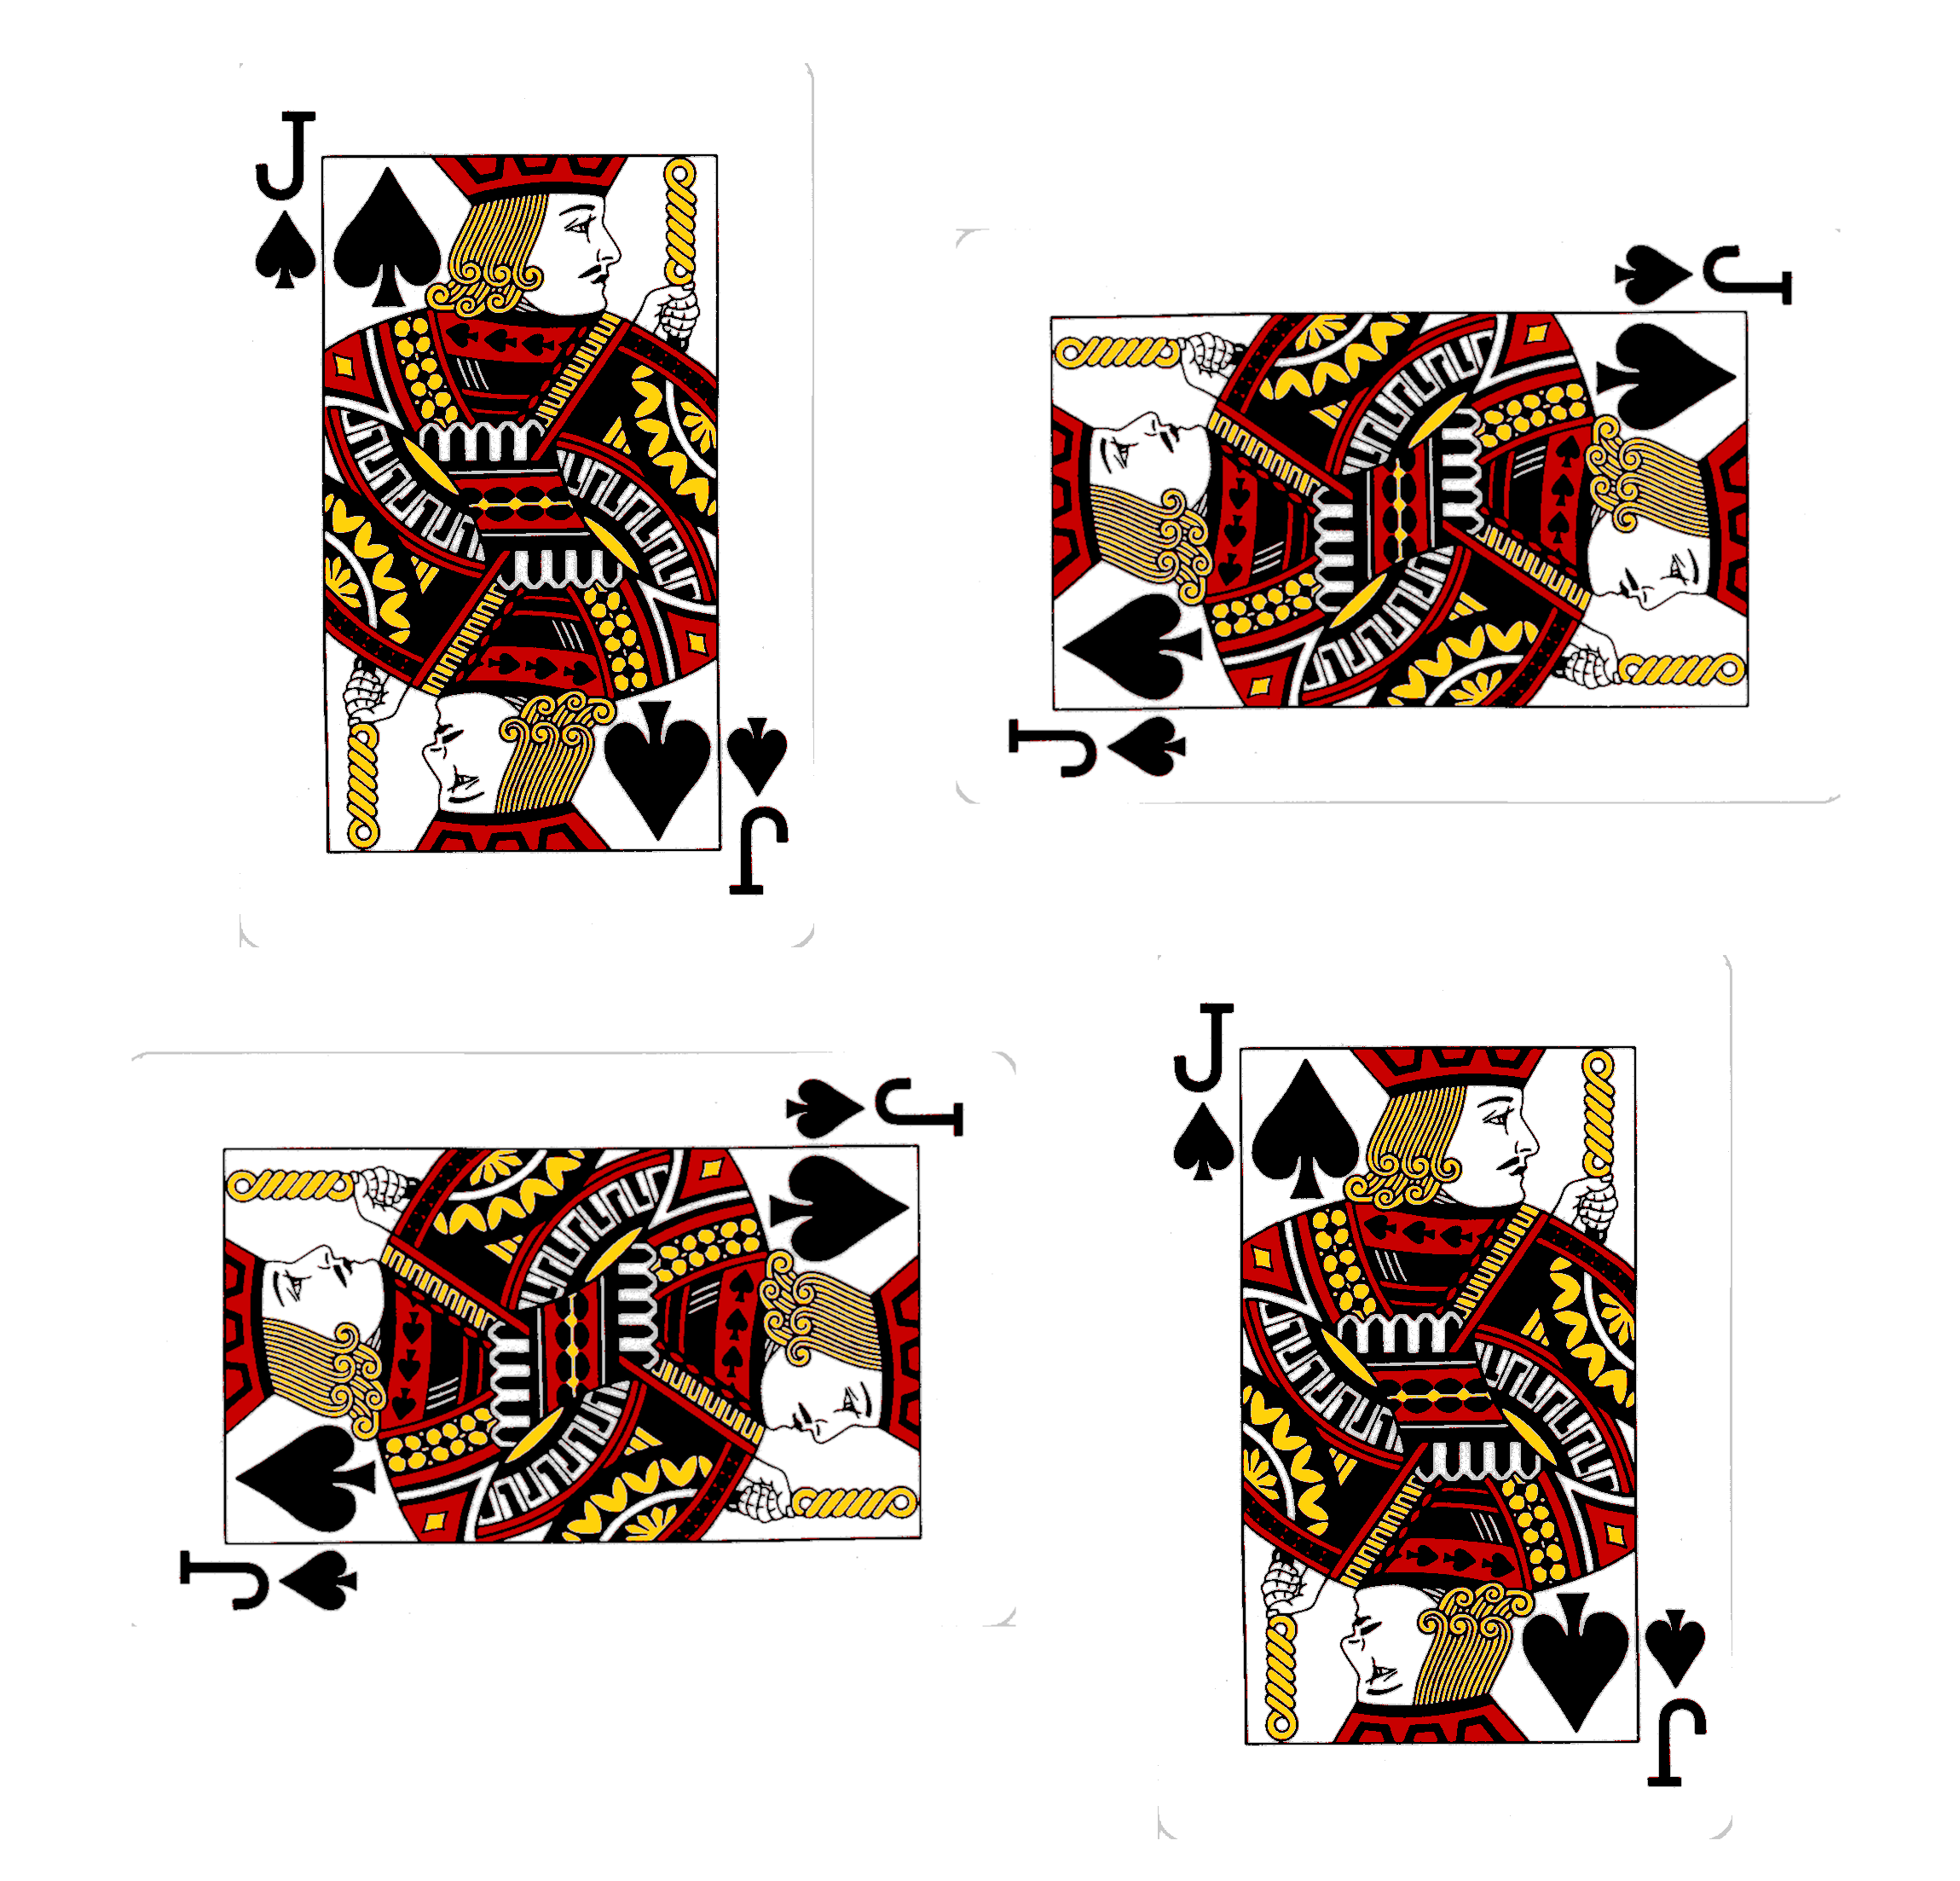
\includegraphics[width=0.75\textwidth,height=0.5\textheight]{../../pictures/images/jacks.png}
	\caption{Here we have applied the group of four rotations to a Jack of spades.
	However, we see that there exists symmetry within the these rotations,
	there are only two distinct rotations, vertical and horizontal. This is because }
\end{figure}

The action of a group on XXX.

\subsection{Symmetries for RL}\label{mdp-homomorphism}

While there are many types of finite group, (cyclic, alternating, ...?) And then there are continuious symmetries, (Lie groups)
Which types of symmetry are important for RL problems?

Let's work through an example, the cart-pole control problem. Your goal is to balance a pole on a cart.
You are allowed to move the cart left or right.

% How hard is it to find these symmetries?
% Are some harder than others?

\begin{figure}[h!]
	\centering
	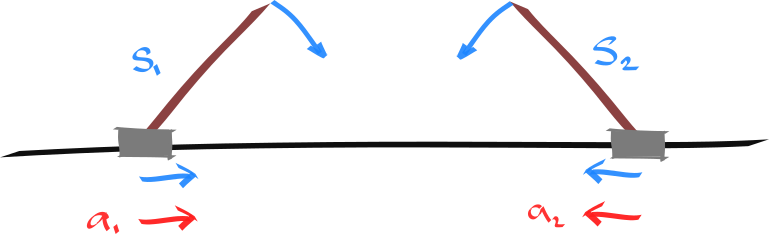
\includegraphics[width=1\textwidth,height=0.25\textheight]{../../pictures/drawings/cart-pole-mirror.png}
	\caption{Two mirror symmetric states of a cart pole. But in what sense are they symmetric?}
\end{figure}

% Need to show this is actually a symmetry, isomorphic to $S_2$?!?
In the case above, the mirrored cart pole is an instance of $S_2$.
The action $f, g$ we apply to the MDP is isomorphism to the simple finite group, $S_2$

Closely related to a homomorphism. See for a definition of a MDP homomorphism that captures symmetries.
% As pointed out in \ref{abstraction}, the notion of an abstraction is captured by a homomorphism.
% So, what would it look like if we had a MDP homomorphism?

\cite{Ravindran2002}

$\mathcal H: \mathcal M\to \mathcal M$.

\begin{align}
P(f(s')|f(s), g_s(a)) = \sum_{s''\in [s']_f} P(s''| a, s) \\
r(f(s), g_s(a)) = r(s, a)
\end{align}

This MDP homomorphism framework is a state-action abstraction, that uses a model based notion of similarity.
However, as pointed out in eariler sections, there are many other possible
notions of abstraction and similarity that make sense for RL. Specifically, the MDP homomorphism framework
could be generalised in the following ways;

\begin{itemize}
\tightlist
  \item temporal symmetries
  \item approximate symmetries
  \item inference of symmetries under uncertainty
  \item complexity measure / inductive bias
\end{itemize}




\subsection{Exploitation} \label{symmetric-exploitation}

\begin{displayquote}
\textit{Once have discovered a symmetry, how might we exploit that knowledge?}
\end{displayquote}

Similar to how we considered how to exploit an abstraction in section \ref{},
let's review some existing methods for exploiting the knowledge of a symmetry. \footnotemark[22]

\footnotetext[22]{Note that, in all of these methods, symmetry provides
advantage over considering just the pairwise similarities. We will return to this later.}

\subsubsection{Exploiting symmetry for efficient control}

If we have a MDP, $M_1$, then solving it via value iteration requires $\mathcal O(\epsilon |S|^2|A|)$ iterations.
However, if we know that there exists symmetries in the state space, then we can 'minimise the model',
by applying the MDP homomorphism $\mathcal H: \mathcal M\to \mathcal M$.
This new, minimised, MDP, $M_2$ has a smaller state space, as $|S_{M_2}| = \frac{|S_{M_1}|}{k}$
and essentially the same dynamics and rewards. Thus we can solve $M_2$, with cost $\mathcal O(\epsilon \frac{|S|^2|A|}{k^2})$
and then lift the solution back to $M_1$. \cite{Dean1997, NARAYANAMURTHY}


\subsubsection{Exploiting symmetry for efficient inference}

There has been a large amount of work (that we are familiar with) exploring
the exploitation of ... See  here for an overview \ref{symmetry-inference}.

The general essence of the idea is \textit{"invariance reduces variance"}. \cite{Chen2019}

\subsubsection{Exploiting symmetry for efficient exploration}

Holtzen et al. \cite{Holtzen2019} show that by grouping together variables according to
the knowledge of a symmetry, they show that \textit{orbit-jump MCMC mixes rapidly in the number of orbits}.
In other words, symmetries allow the efficient estimation of distributions.
% Want to demonstrate this.
% {\color{red}TODO max ent + abstraction experiments}

\begin{center}\rule{0.5\linewidth}{\linethickness}\end{center}

All of these methods rely on a similar type of argument. Picking a representative
of a partition and only using that one. Averaging over orbits. ...

\subsection{Discovery}

% This is about generalising using an inductive bias towards symmetry.

Symmetry is a stricter notion of similarity. How can it be discovered?

Relationship to disentanglement. \cite{Higgins2018} which makes a lot of sense because ...

Connection to causal hierarchy. Cite Pearl. Association, intervention, counterfactuals.
Also recently noted by \cite{Caselles-Dupre2019}, ... where they assume that
the group actions are the actions of the RL environment.
This doesn't really make sense. Also, will miss many symmetries like ???

A couple parts. Discovery of symmetries, exploration of the knowledge of symmetries.

Unsupervised discovery. Not much success yet. Only when using some kind of supervised signal.

\cite{Ho2019a, Lim2019, Cubuk2018, Cubuk2019}
Discover which symmetries apply to a given domain, and at what magnitude.
The optimisation problem becomes one of picking the probability of each op and its magnitude.
There is a small set of ops (aka symmetries) that are given:
\textit{Identity, AutoContrast, Equalize, Rotate, Solarize, Color, Posterize, Contrast,
	Brightness, Sharpness, ShearX, ShearY, TranslateX, TranslateY.}
Uses validation error as a reward for learning.


\subsubsection{Inferring symmetries from experience}

% How easy is it to solve this symmetry inference problem?

% HOW?!

What does this buy us? If have sufficient data to tell us that $x$ and $y$ are
similar, say that they are mirror images of each other.
As an unsupervised pre-training step. Then apply and share labels and learn more quickly?
What else can $x$ tell us about $y$?

\cite{Yang2019}

Or end to end? As we get more certain that x and y are similar, we more strongly
encourage their symmetry through one of the methods outlined above.
Is it possible (/easier) to learn that x and y are similar (in terms of their labels) before (accurately) learning their labels.



Want to have an inductive bias towards simpler symmetries. But, how can we do this without needing to represent all possible symmetries?
A solution rejection sampling??


%
% - What about symmetries that are products of subgroups? $S = Z_2 \times Z_3$?
% Are they easier to infer?
% - Within the same $n$. Is there a notion of more or less complex group structures??
% - Need to show that NNs dont have the right symmetric inductive bias. They dont generalise. !!!

% Examples

% - Knowing that; range $= [0,360)$, and $0, 45, 90, 135, 180$, all are similar. I guess that we are in cyclic group $8$ and therefore $225, 270, 315$ are also similar. Key is that I know that $0, 45, 90, 135, 180$ are related by $0+0, 0+45, 0+45+45, 0+45+45+45, 0+45+45+45+45$.
% - Cart pole. $V^{\pi(s, a)}(s') = V^{\pi(-s, -a)}(-s') \forall s'$.


\subsubsection{Invariants}

Symmetries can be uniquely characterised by their invariants \cite{PeterOlver1999}.
What are the interesting invariants of MDPs? And how do they ???
But, what does this symmetry imply about other quantities of interest for RL?

Invariance, $f(g(x)) = f(x)$, equivariance, $f(g(x)) = g(f(x))$.

In general we want to know;

\begin{itemize}
	\tightlist
	\item We have $n$ different 'symmetries'. But are they really different?
	\item Which symmetries share some invariants?
	\item Which invariants uniquely characterise this symmetry?
\end{itemize}

With this knowledge, we could identify symmetries via their invariants!?!
We can observe invariant properties. (not clear to me how you observe a symmetry!?)

We briefly explore this in \ref{game-invariants}.


\subsection{Inductive bias towards seeing symmetry}

In the introduction to abstractions for RL we considered learning similarities
to build an abstraction. But, learning pairwise similarities does not give
you the ability to generalise. To generalise you need other priors. For example;
CNNs generalise because they implicitly encode priors for smoothness and explicitly for locality. (ref)

Another potentially useful prior is symmetry: \textit{"We believe it is likely that
the problems we are given have some symmetry within them."}

The intuition is, this symmetry prior helps us generalise because, we can guess
a symmetry that matches the observed pairwise similarities. This symmetry might
require that other pairs to be similar (because of the closed natured of groups).
Thus, we can generalise knowledge from some pairwise similarities to others
pairwise similarities (assuming the prior is correct).

\subsubsection{RL as inference}

Need to introduce RL as an inference problem. Which we can add priors to.


\subsubsection{Bayesian priors}

Then motivate these priors. WANT GENERALISATION! But aint gonna get it from the
methods above.

% The problem is the cost of inferring symmetry

% Would prefer to be able to sample easily constructible models. But this would require some sort choice of the family?


We have a prior belief that symmetric $\tau, r$ should be more likely, this is captured by the distribution $P_S(\tau, r)$.
MAP estimate of the data is $P(\tau_{\theta}, r_{\phi}| D) = \frac{P(D | \tau_{\theta}, r_{\phi})P_S(\tau_{\theta}, r_{\phi})}{P(D)}$.

But, how can we construct $P_S(\tau_{\theta}, r_{\phi})$?
Actually, we dont need to construct it, we only need samples!!?
Then we can apply, grad descent, and the noise from the samples will average out!?


Alternatively. The data generates a distribution over likely abstractions.
$P(A|D) = \frac{P(D|A)P(A)}{P(D)}$??? Where the data here is the pairwise similarities?!?
The key is $P(A)$. Which abstractions should we encourage? Coarser is better.
Should be symmetric matrices. Should be full rank. What about identity, should also be likely?
Identity is no symmetries.

% \subsubsection{Langevin dynamics}
%
% Clip to nearest symmetric abstraction.
%
% \begin{align}
% \mathop{\text{argmin}}_{\theta} D(\bar \theta, \theta)
% \end{align}
%
% Where $\bar \theta$ is the nearest symmetric set of parameters.
%
% \begin{align}
% \theta = \theta_t - \eta \nabla_\theta \mathcal S(\theta) + w
% \end{align}
%
% Langevin dynamics. Where $w$ is sampled from some noise distribution.
% Therefore, we get a distribution over $\theta$.
% Only do a few iterations, so we sample $\theta$ that are near by!?!?
% The $\nabla_\theta \mathcal S(\theta)$ pulls us towards symmetric parameters.
%
% Need a differentiable measure of symmetry.!?
% If I actually find this, we can just use it as a regulariser..!?!?!?


\subsubsection{A measure of the symmetry of an MDP}

The size of the automorphism group.
Relax to measure how close we are to ...?


\subsubsection{Thompson sampling} \label{thompson-sampling}

{\color{red}TODO need to introduce this framework}

SARSA plus thompson sampling. Does this really work? Want to test.

\begin{algorithm}
	\caption{Thompson sampling}
	\begin{algorithmic}[1]

		\Procedure{TS}{$\gamma$}
		\State $\pi_t \sim \mathcal U(\Pi)$
		\While{not converged}
		\State $\tilde P, \tilde r \sim P_{\theta}(\cdot)$
		\State $Q_{t+1} =  r + \gamma P Q_t$ \Comment{Bellman operator}
		\State $\theta = \nabla_{\theta} P_{\theta}(P, r)$ \Comment{Max likelihood}

		\EndWhile
		\State \algorithmicreturn{ $\pi$}
		\EndProcedure

	\end{algorithmic}
\end{algorithm}

The way we parameterise the distribution over possible models (/ MDPs), $\theta$, has implicit inductive biases about the true structure of the model.
A way to add explicit inductive biases is via importance (/ rejection) sampling.

We can encourage the model to be more symmetric!?
How much computation does this cost?

But. How can we construct the distribution? We want to be able to take samples
from it.

Ok. Great we have this inductive bias. But it doesnt help exploration in the way I want it to...
The parameters we have learned are close to being symmetric in some way. So the complexity measure alters the likelihoods and makes the symmetric version the most probable.
How does this help exploration? More likely to sample the true model / a symmetric one. Need to be able to exploit this symmetry.

This solves the efficient inference problem. Not efficient exploration... How can we get both?
Sample an abstraction then lift it to the original MDP?!


Thompson sampling from estimates of similarity / symmetry.
\begin{enumerate}
	\tightlist
	\item Keep estimate of similarity. $\chi(x_i, x_j)_{t+1} = \chi(x_i, x_j)_t + ?$
	\item Construct distribution over likely abstractions $P(x_i = x_j) \propto e^{\chi(x_i, x_j)_t}$. $\mathcal F = P(f|\chi_t)$
	\item Sample an abstraction. $f\sim \mathcal F$
	\item Reduce the MDP $M' = f(M)$
\end{enumerate}


For now just assume we have an accurate estimate of the model.
What does acting optimally wrt the reduced model mean for exploration and convergence??


% How to reason about the tradeoff between symmetry and fitting the data!?.
